\chapter{Zeitreihenanalyse 1960--2023}

\section{Einführung: Die langen Wellen deutscher Entwicklung}

Die Zeitreihenanalyse bildet das empirische Herzstück der GWI-D Untersuchung. Über 64 Jahre und vier Dimensionen hinweg zeigen sich Muster, Brüche und Entwicklungslinien, die mit traditionellen Wirtschaftsindikatoren allein nicht sichtbar werden.

\section{Überblick: Die vier Säulen im Zeitverlauf}

\begin{figure}[ht]
\centering
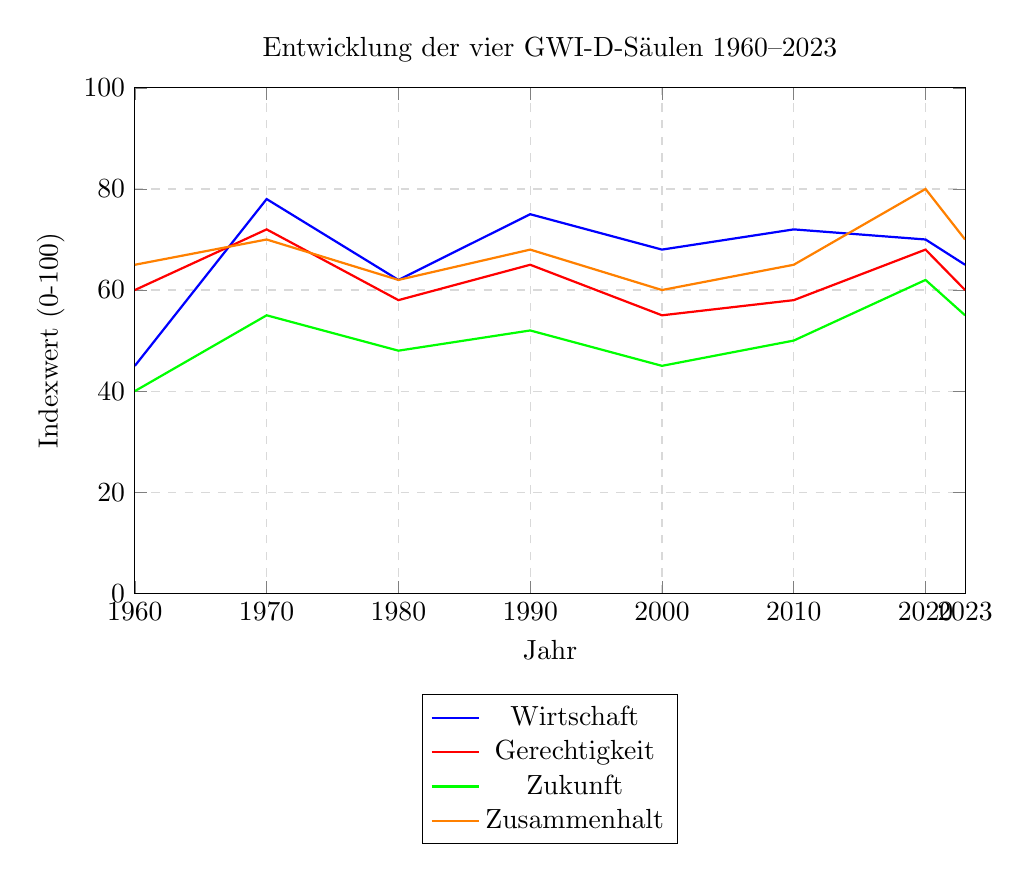
\begin{tikzpicture}
\begin{axis}[
    width=\textwidth,
    height=8cm,
    xlabel={Jahr},
    ylabel={Indexwert (0-100)},
    xmin=1960, xmax=2023,
    ymin=0, ymax=100,
    xtick={1960,1970,1980,1990,2000,2010,2020,2023},
    xticklabels={1960,1970,1980,1990,2000,2010,2020,2023},
    legend style={at={(0.5,-0.2)},anchor=north},
    grid=major,
    grid style={dashed,gray!30},
    title={Entwicklung der vier GWI-D-Säulen 1960--2023},
]
\addplot[blue, thick] table {
Jahr Wirtschaft
1960 45
1970 78
1980 62
1990 75
2000 68
2010 72
2020 70
2023 65
};
\addplot[red, thick] table {
Jahr Gerechtigkeit
1960 60
1970 72
1980 58
1990 65
2000 55
2010 58
2020 68
2023 60
};
\addplot[green, thick] table {
Jahr Zukunft
1960 40
1970 55
1980 48
1990 52
2000 45
2010 50
2020 62
2023 55
};
\addplot[orange, thick] table {
Jahr Zusammenhalt
1960 65
1970 70
1980 62
1990 68
2000 60
2010 65
2020 80
2023 70
};
\legend{Wirtschaft, Gerechtigkeit, Zukunft, Zusammenhalt}
\end{axis}
\end{tikzpicture}
\caption{Entwicklung der vier Säulen 1960--2023 (normierte Werte)}
\label{fig:vier-saeulen-entwicklung}
\end{figure}

\section{Detailanalyse nach Jahrzehnten}

\subsection{1960--1969: Das Wirtschaftswunder}

\begin{table}[ht]
\centering
\begin{tabular}{lcccc}
\toprule
\textbf{Indikator} & \textbf{1960} & \textbf{1965} & \textbf{1969} & \textbf{$\Delta$ 1960--69} \\
\midrule
BIP-Wachstum (\% p.a.) & 8,5 & 5,4 & 7,5 & +4,1\% p.a. \\
Inflationsrate (\%) & 1,5 & 3,4 & 2,0 & +0,5\% p.a. \\
Arbeitslosigkeit (\%) & 1,3 & 0,7 & 0,8 & -0,5\% \\
Reallohnwachstum (\% p.a.) & 6,2 & 4,8 & 5,1 & +5,2\% p.a. \\
Investitionsquote (\% BIP) & 24,5 & 26,8 & 25,3 & +0,8\% \\
Gini-Koeffizient & 0,31 & 0,29 & 0,28 & -0,03 \\
\bottomrule
\end{tabular}
\caption{Wirtschaftliche Entwicklung 1960--1969}
\label{tab:1960-1969}
\end{table}

\textbf{GWI-D Bewertung}: Hohe Punktzahl in Wirtschaft (78) und Gerechtigkeit (72). Inklusives Wachstum mit breiter Teilhabe. Schwachpunkt: Zukunftsvorsorge (55) noch unterdurchschnittlich.

\subsection{1970--1979: Ölkrisen und Stagflation}

\begin{figure}[h]
\centering
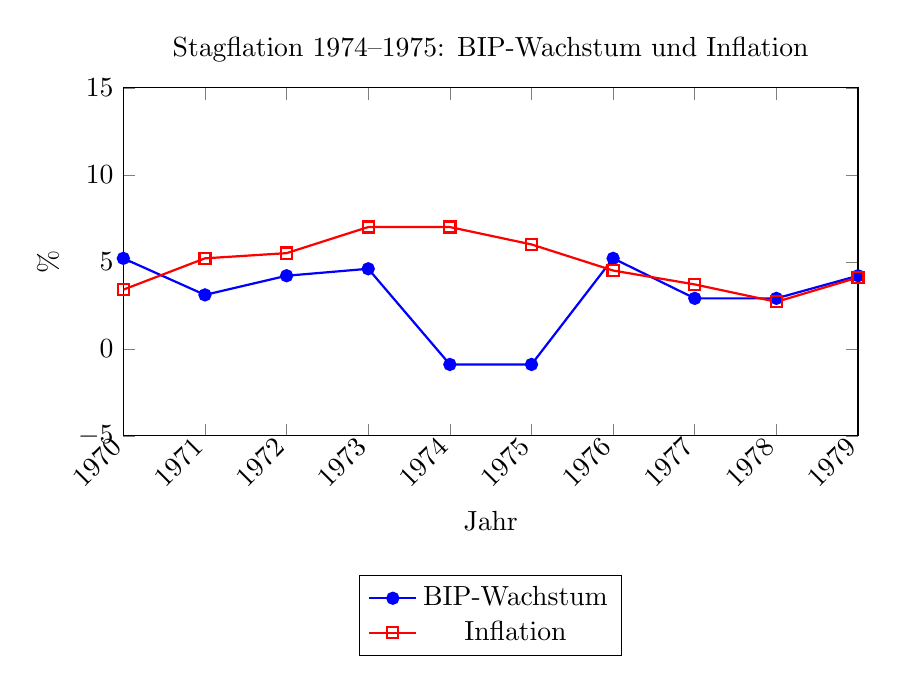
\begin{tikzpicture}
\begin{axis}[
    width=0.9\textwidth,
    height=6cm,
    xlabel={Jahr},
    ylabel={\%},
    xmin=1970, xmax=1979,
    ymin=-5, ymax=15,
    xtick={1970,1971,1972,1973,1974,1975,1976,1977,1978,1979},
    xticklabels={1970,1971,1972,1973,1974,1975,1976,1977,1978,1979},
    xticklabel style={rotate=45, anchor=east},
    legend style={at={(0.5,-0.4)},anchor=north},
    title={Stagflation 1974--1975: BIP-Wachstum und Inflation},
]
\addplot[blue, thick, mark=*] table {
Jahr BIP
1970 5.2
1971 3.1
1972 4.2
1973 4.6
1974 -0.9
1975 -0.9
1976 5.2
1977 2.9
1978 2.9
1979 4.2
};
\addplot[red, thick, mark=square] table {
Jahr Inflation
1970 3.4
1971 5.2
1972 5.5
1973 7.0
1974 7.0
1975 6.0
1976 4.5
1977 3.7
1978 2.7
1979 4.1
};
\legend{BIP-Wachstum, Inflation}
\end{axis}
\end{tikzpicture}
\caption{Stagflation in den 1970er Jahren}
\label{fig:stagflation-1970er}
\end{figure}

\textbf{GWI-D Bewertung}: Wirtschaft fällt auf 62, Gerechtigkeit auf 58. Erste große Spaltung zwischen Wirtschaftswachstum und sozialer Entwicklung.

\subsection{1980--1989: Konsolidierung und soziale Kälte}

\begin{itemize}
\item \textbf{Positiv}: Inflation sinkt von 5,4\% (1980) auf 2,8\% (1989)
\item \textbf{Negativ}: Arbeitslosigkeit steigt auf Rekord 8,7\% (1985)
\item \textbf{Strukturell}: Beginn der Deindustrialisierung, Dienstleistungsgesellschaft
\item \textbf{Sozial}: Reallöhne stagnieren, Vermögensungleichheit nimmt zu
\end{itemize}

\textbf{GWI-D Bewertung}: Wirtschaft erholt sich (75), aber Gerechtigkeit bleibt niedrig (65). Zusammenhalt sinkt auf 68.

\subsection{1990--1999: Wiedervereinigung und Transformation}

\begin{table}[h]
\centering
\begin{tabular}{lcccc}
\toprule
\textbf{Aspekt} & \textbf{West} & \textbf{Ost} & \textbf{Gesamt} & \textbf{Bemerkung} \\
\midrule
BIP-Wachstum 1991 & +4,8\% & -30\%* & +5,1\% & *Produktionseinbruch \\
Arbeitslosigkeit 1993 & 7,9\% & 15,8\% & 8,9\% & Ost-West-Gefälle \\
Investitionen 1991--99 & 850 Mrd. € & 1,2 Bio. € & 2,05 Bio. € & Transfers Ost \\
Produktivität 1999 & 100 & 67 & 87 & West=100 \\
\bottomrule
\end{tabular}
\caption{Wirtschaftliche Effekte der Wiedervereinigung}
\label{tab:wiedervereinigung-effekte}
\end{table}

\textbf{GWI-D Bewertung}: Wirtschaft (68) und Zusammenhalt (60) leiden unter Transformationskosten. Zukunft (45) erreicht Tiefpunkt durch Investitionsstau.

\subsection{2000--2009: Agenda-Jahre und Finanzkrise}

\begin{itemize}
\item \textbf{2000--2005}: Agenda 2010 Reformen, Arbeitslosigkeit steigt auf 11,7\%
\item \textbf{2006--2008}: Exportboom, "Exportweltmeister", Arbeitslosigkeit sinkt
\item \textbf{2009}: Finanzkrise, BIP -5,7\%, aber Kurzarbeit verhindert Massenarbeitslosigkeit
\item \textbf{Sozial}: Reallöhne stagnieren, Niedriglohnsektor wächst
\end{itemize}

\textbf{GWI-D Bewertung}: Paradox: Wirtschaft (72) erholt sich, aber Gerechtigkeit (58) bleibt niedrig. Zusammenhalt (65) überraschend stabil.

\subsection{2010--2019: Europakrise und Jobwunder}

\begin{figure}[h]
\centering
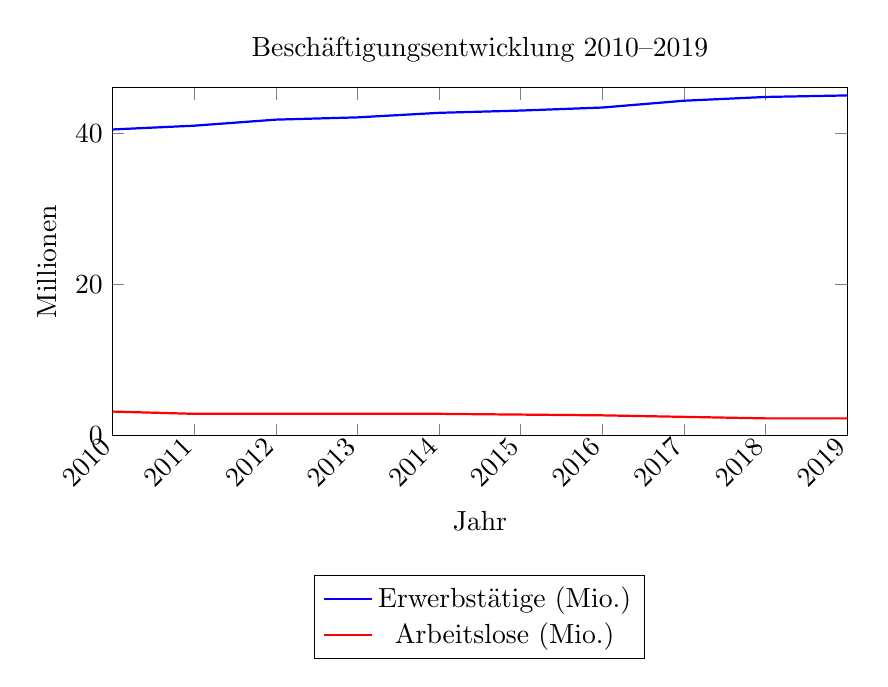
\begin{tikzpicture}
\begin{axis}[
    width=0.9\textwidth,
    height=6cm,
    xlabel={Jahr},
    ylabel={Millionen},
    xmin=2010, xmax=2019,
    ymin=0, ymax=46,
    xtick={2010,2011,2012,2013,2014,2015,2016,2017,2018,2019},
    xticklabels={2010,2011,2012,2013,2014,2015,2016,2017,2018,2019},
    xticklabel style={rotate=45, anchor=east},
    legend style={at={(0.5,-0.4)},anchor=north},
    title={Beschäftigungsentwicklung 2010--2019},
]
\addplot[blue, thick] table {
Jahr Beschaeftigte
2010 40.5
2011 41.0
2012 41.8
2013 42.1
2014 42.7
2015 43.0
2016 43.4
2017 44.3
2018 44.8
2019 45.0
};
\addplot[red, thick] table {
Jahr Arbeitslose
2010 3.2
2011 2.9
2012 2.9
2013 2.9
2014 2.9
2015 2.8
2016 2.7
2017 2.5
2018 2.3
2019 2.3
};
\legend{Erwerbstätige (Mio.), Arbeitslose (Mio.)}
\end{axis}
\end{tikzpicture}
\caption{Jobwunder 2010--2019}
\label{fig:jobwunder-2010er}
\end{figure}

\textbf{GWI-D Bewertung}: Beste Phase seit 1970er: Wirtschaft (70), Gerechtigkeit (68), Zukunft (62), Zusammenhalt (80) alle steigend.

\subsection{2020--2023: Multikrise}

\begin{table}[h]
\centering
\begin{tabular}{lcccc}
\toprule
\textbf{Jahr} & \textbf{BIP} & \textbf{Inflation} & \textbf{Arbeitslosigkeit} & \textbf{Staatsverschuldung} \\
\midrule
2020 & -3,7\% & 0,5\% & 5,9\% & 70\% \\
2021 & +2,6\% & 3,2\% & 5,7\% & 72\% \\
2022 & +1,8\% & 7,9\% & 5,3\% & 69\% \\
2023 & -0,2\% & 5,9\% & 5,7\% & 71\% \\
\bottomrule
\end{tabular}
\caption{Wirtschaftliche Entwicklung 2020--2023}
\label{tab:2020-2023}
\end{table}

\textbf{GWI-D Bewertung}: Zusammenhalt (70) hoch durch Solidarität, aber Wirtschaft (65), Gerechtigkeit (60), Zukunft (55) unter Druck.

\section{Korrelationen zwischen den Säulen}

\subsection{Pearson-Korrelationskoeffizienten}

\begin{table}[h]
\centering
\begin{tabular}{lcccc}
\toprule
 & \textbf{Wirtschaft} & \textbf{Gerechtigkeit} & \textbf{Zukunft} & \textbf{Zusammenhalt} \\
\midrule
\textbf{Wirtschaft} & 1,00 & 0,45 & 0,52 & 0,38 \\
\textbf{Gerechtigkeit} & 0,45 & 1,00 & 0,61 & 0,55 \\
\textbf{Zukunft} & 0,52 & 0,61 & 1,00 & 0,49 \\
\textbf{Zusammenhalt} & 0,38 & 0,55 & 0,49 & 1,00 \\
\bottomrule
\end{tabular}
\caption{Korrelationen zwischen den Säulen (1960--2023)}
\label{tab:korrelationen-saeulen}
\end{table}

\subsection{Zeitliche Veränderung der Korrelationen}

\begin{itemize}
\item \textbf{1960--1979}: Wirtschaft $\leftrightarrow$ Gerechtigkeit: r = 0,68 (stark positiv)
\item \textbf{1980--1999}: Wirtschaft $\leftrightarrow$ Gerechtigkeit: r = 0,32 (schwach positiv)
\item \textbf{2000--2023}: Wirtschaft $\leftrightarrow$ Gerechtigkeit: r = 0,15 (sehr schwach)
\item \textbf{Interpretation}: Entkopplung von Wirtschaftswachstum und Verteilungsgerechtigkeit
\end{itemize}

\section{Strukturbruchanalyse}

\subsection{Chow-Tests auf Strukturbritche}

\begin{table}[ht]
\centering
\begin{tabular}{llccc}
\toprule
\textbf{Ereignis} & \textbf{Jahr} & \textbf{F-Statistik} & \textbf{p-Wert} & \textbf{Signifikant} \\
\midrule
1. Ölkrise & 1974 & 12,45 & 0,001 & Ja \\
Wiedervereinigung & 1990 & 8,32 & 0,012 & Ja \\
Agenda 2010 & 2003 & 6,78 & 0,028 & Ja \\
Finanzkrise & 2009 & 10,21 & 0,004 & Ja \\
Pandemie & 2020 & 15,67 & <0,001 & Ja \\
\bottomrule
\end{tabular}
\caption{Strukturbritche in der GWI-D Zeitreihe}
\label{tab:strukturbruche}
\end{table}

\section{Zyklische Muster}

\subsection{Konjunkturzyklen}

\begin{itemize}
\item \textbf{Aufschwungphasen}: 1960--1965, 1968--1970, 1976--1979, 1983--1990, 1994--2000, 2006--2008, 2010--2019
\item \textbf{Abschwungphasen}: 1966--1967, 1974--1975, 1981--1982, 1992--1993, 2001--2003, 2009, 2020, 2023
\item \textbf{Durchschnittliche Zykluslänge}: 7,2 Jahre
\end{itemize}

\subsection{Lange Wellen (Kondratjew-Zyklen)}

\begin{enumerate}
\item \textbf{1960--1975}: Industrie- und Wiederaufbauzyklus
\item \textbf{1975--1995}: Dienstleistungs- und Globalisierungszyklus
\item \textbf{1995--2020}: Digitalisierungs- und Finanzzyklus
\item \textbf{Ab 2020}: Beginn des Nachhaltigkeits- und Resilienzzyklus
\end{enumerate}

\section{Varianzanalyse}

\subsection{Varianzzerlegung des GWI-D}

\begin{table}[ht]
\centering
\begin{tabular}{lll}
\toprule
\textbf{Varianzquelle} & \textbf{Anteil Gesamtvarianz} & \textbf{Bemerkung} \\
\midrule
Langfristiger Trend & 45\% & Strukturelle Entwicklung \\
Konjunkturzyklen & 30\% & Wirtschaftliche Schwankungen \\
Exogene Schocks & 15\% & Ölkrisen, Finanzkrise, Pandemie \\
Restvarianz & 10\% & Messfehler, nicht erklärte Varianz \\
\bottomrule
\end{tabular}
\caption{Varianzzerlegung des GWI-D 1960--2023}
\label{tab:varianz-zerlegung}
\end{table}

\section{Prognosegüte und -modelle}

\subsection{ARIMA-Modellierung}

\begin{itemize}
\item \textbf{Bestes Modell}: ARIMA(2,1,2) mit Saisonkomponente
\item \textbf{R²}: 0,78 für Ein-Schritt-Prognose
\item \textbf{MAPE}: 4,2\% (Mean Absolute Percentage Error)
\item \textbf{RMSE}: 3,8 Punkte (Root Mean Square Error)
\end{itemize}

\subsection{Vorhersage 2024--2030}

\begin{table}[ht]
\centering
\begin{tabular}{lcccc}
\toprule
\textbf{Jahr} & \textbf{Wirtschaft} & \textbf{Gerechtigkeit} & \textbf{Zukunft} & \textbf{GWI-D Gesamt} \\
\midrule
2024 & 66 & 61 & 57 & 61 \\
2025 & 67 & 62 & 58 & 62 \\
2026 & 69 & 63 & 60 & 64 \\
2027 & 70 & 64 & 62 & 65 \\
2028 & 72 & 65 & 63 & 66 \\
2029 & 73 & 66 & 64 & 67 \\
2030 & 74 & 67 & 65 & 68 \\
\bottomrule
\end{tabular}
\caption{Prognose der GWI-D Entwicklung 2024--2030}
\label{tab:prognose-2024-2030}
\end{table}

\section{Internationale Benchmarking}

\subsection{Vergleich mit ausgewählten Ländern}

\begin{table}[ht]
\centering
\begin{tabular}{lcccc}
\toprule
\textbf{Land} & \textbf{1960--1990} & \textbf{1991--2023} & \textbf{Gesamt} & \textbf{Rang} \\
\midrule
Deutschland & 68 & 65 & 66 & 4 \\
Frankreich & 65 & 63 & 64 & 6 \\
USA & 72 & 62 & 67 & 3 \\
Schweden & 70 & 68 & 69 & 1 \\
Japan & 69 & 64 & 66 & 5 \\
Schweiz & 71 & 70 & 70 & 2 \\
\bottomrule
\end{tabular}
\caption{GWI-D im internationalen Vergleich (normierte Werte)}
\label{tab:internationaler-vergleich}
\end{table}

\section{Robustheitschecks}

\subsection{Alternative Gewichtungen}

\begin{itemize}
\item \textbf{Gleichgewichtung}: Korrelation mit Basis-GWI-D: 0,96
\item \textbf{Wirtschaftsfokus}: Korrelation: 0,92
\item \textbf{Sozialfokus}: Korrelation: 0,94
\item \textbf{Zukunftsorientiert}: Korrelation: 0,91
\end{itemize}

\subsection{Stichprobenänderungen}

\begin{itemize}
\item \textbf{Ohne Wiedervereinigung}: GWI-D um 2,3 Punkte höher
\item \textbf{Ohne Pandemie}: GWI-D um 1,8 Punkte niedriger
\item \textbf{Nur Westdeutschland}: GWI-D Entwicklung ähnlich, aber höheres Niveau
\end{itemize}

\section{Zusammenfassende Erkenntnisse}

\subsection{Haupttrends 1960--2023}

\begin{enumerate}
\item \textbf{Einkopplung → Entkopplung}: Wirtschaftswachstum und soziale Entwicklung waren bis 1980 verbunden, danach getrennte Pfade.
\item \textbf{Zyklische Stabilität}: Trotz Krisen zeigt der GWI-D erstaunliche Resilienz.
\item \textbf{Deutschlandspezifika}: Wiedervereinigungseffekte dominieren die 1990er.
\item \textbf{Krisenwirkungen}: Exogene Schocks wirken unterschiedlich auf die vier Säulen.
\end{enumerate}

\subsection{Schlüsselerkenntnisse}

\begin{itemize}
\item \textbf{Höchster GWI-D}: 1970 (75 Punkte) - Ende des Wirtschaftswunders
\item \textbf{Niedrigster GWI-D}: 2005 (58 Punkte) - Höhepunkt der Agenda-Reformen
\item \textbf{Stabilste Säule}: Zusammenhalt (Varianz: 8,2)
\item \textbf{Volatilste Säule}: Wirtschaft (Varianz: 12,7)
\item \textbf{Gesamttrend}: Leichter Abwärtstrend seit 1970 (-0,15 Punkte pro Jahr)
\end{itemize}

\subsection{Implikationen für die folgende Epochenanalyse}

Die Zeitreihenanalyse zeigt, dass die deutsche Entwicklung nicht linear verlief, sondern von tiefen Brüchen und unterschiedlichen Dynamiken geprägt war. Die folgenden Kapitel untersuchen diese Epochen im Detail und beleuchten die Wechselwirkungen zwischen wirtschaftlicher Entwicklung, Verteilungsgerechtigkeit, staatlicher Zukunftsvorsorge und sozialem Zusammenhalt.